\documentclass{article}
\usepackage{amsmath,amssymb,amsthm}
\usepackage{enumerate}
\usepackage{mathtools}
\usepackage{graphicx}
\usepackage{caption}
\usepackage{bm}
\newtheorem{theorem}{Theorem}
\newtheorem{question}[theorem]{Question}
\newtheorem{answer}[theorem]{Solution}
\newcommand{\myvec}[1]{\ensuremath{\begin{pmatrix}#1\end{pmatrix}}}
\let\vec\mathbf
\begin{document}
\begin{question}
Show that the vectors $\myvec{-2 \\ +1 \\ -1}$,$\myvec{+2 \\ -1 \\ +1}$ and $\myvec{+1\\-3\\-5}$
form the vertices of a right angled triangle.
\end{question}
Solution. Let $\vec{A}$,$\vec{B}$  and $\vec{C}$ be given vectors such that:
\begin{equation}
\vec{A} = \myvec{-2 \\ +1 \\ -1}, \quad \vec{B}=\myvec{+2 \\ -1 \\ +1} \quad and \quad
\vec{C}= \myvec{+1\\-3\\-5}	
\end{equation}
Given below is the figure formed by $\vec{A}$, $\vec{B}$ and $\vec{C}$.

\begin{figure}[!htb]
	
	\centering
	
	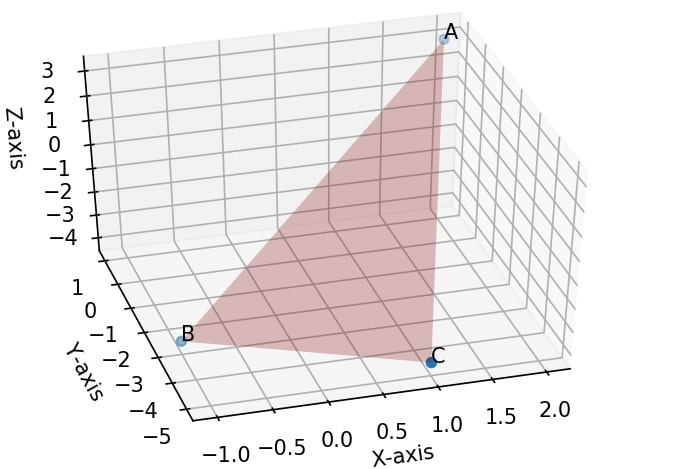
\includegraphics[width=\columnwidth]{assignment1fig-1.jpg}
	
	\caption{\label{fig1}}
	
	\label{fig:}
	
\end{figure}
Clearly, $\vec{A}\vec{B}\vec{C}$ is a triangle.
To prove, the $\triangle ABC$ is a right triangle, we need to calculate the inner product of all the below vectors and check if any one of them is 0:
\begin{align}
	(\vec{A} -\vec{C})^T (\vec{B}-\vec{C}) = (-1 \quad+3 \quad +5) \myvec{-2 \\ +1 \\ -1}  = 00 \\
	(\vec{A} -\vec{B})^T (\vec{C}-\vec{B})
	 = (+1 \quad +2 \quad +6) \myvec{+2 \\ -1 \\ +1} = 06 \\
    (\vec{B} -\vec{A})^T (\vec{C}-\vec{A}) = (-1\quad-2 \quad-6) \myvec{+1\\-3\\-5} = 35 
\end{align}
Clearly, from ($2$) we can see that $\triangle$ABC is right angled at C.
\end{document}
